%%%%%%%%%%%%%%%%%%%%%%%%%%%%%%%%%%%%%%%%%
% Short Sectioned Assignment LaTeX Template Version 1.0 (5/5/12)
% This template has been downloaded from: http://www.LaTeXTemplates.com
% Original author:  Frits Wenneker (http://www.howtotex.com)
% License: CC BY-NC-SA 3.0 (http://creativecommons.org/licenses/by-nc-sa/3.0/)
%%%%%%%%%%%%%%%%%%%%%%%%%%%%%%%%%%%%%%%%%

%----------------------------------------------------------------------------------------
%	PACKAGES AND OTHER DOCUMENT CONFIGURATIONS
%----------------------------------------------------------------------------------------

\documentclass[paper=a4, fontsize=11pt]{scrartcl} % A4 paper and 11pt font size

% ---- Entrada y salida de texto -----

\usepackage[T1]{fontenc} % Use 8-bit encoding that has 256 glyphs
\usepackage[utf8]{inputenc}
%\usepackage{fourier} % Use the Adobe Utopia font for the document - comment this line to return to the LaTeX default

% ---- Idioma --------

\usepackage[spanish, es-tabla]{babel} % Selecciona el español para palabras introducidas automáticamente, p.ej. "septiembre" en la fecha y especifica que se use la palabra Tabla en vez de Cuadro

% ---- Otros paquetes ----

\usepackage{url} % ,href} %para incluir URLs e hipervínculos dentro del texto (aunque hay que instalar href)
\usepackage{amsmath,amsfonts,amsthm} % Math packages
%\usepackage{graphics,graphicx, floatrow} %para incluir imágenes y notas en las imágenes
\usepackage{graphics,graphicx, float} %para incluir imágenes y colocarlas

% Para hacer tablas comlejas
%\usepackage{multirow}
%\usepackage{threeparttable}

%\usepackage{sectsty} % Allows customizing section commands
%\allsectionsfont{\centering \normalfont\scshape} % Make all sections centered, the default font and small caps

\usepackage{fancyhdr} % Custom headers and footers
\pagestyle{fancyplain} % Makes all pages in the document conform to the custom headers and footers
\fancyhead{} % No page header - if you want one, create it in the same way as the footers below
\fancyfoot[L]{} % Empty left footer
\fancyfoot[C]{} % Empty center footer
\fancyfoot[R]{\thepage} % Page numbering for right footer
\renewcommand{\headrulewidth}{0pt} % Remove header underlines
\renewcommand{\footrulewidth}{0pt} % Remove footer underlines
\setlength{\headheight}{13.6pt} % Customize the height of the header

\numberwithin{equation}{section} % Number equations within sections (i.e. 1.1, 1.2, 2.1, 2.2 instead of 1, 2, 3, 4)
\numberwithin{figure}{section} % Number figures within sections (i.e. 1.1, 1.2, 2.1, 2.2 instead of 1, 2, 3, 4)
\numberwithin{table}{section} % Number tables within sections (i.e. 1.1, 1.2, 2.1, 2.2 instead of 1, 2, 3, 4)

\setlength\parindent{0pt} % Removes all indentation from paragraphs - comment this line for an assignment with lots of text

\newcommand{\horrule}[1]{\rule{\linewidth}{#1}} % Create horizontal rule command with 1 argument of height



% Para usar urls
\usepackage{hyperref}

%----------------------------------------------------------------------------------------
%	TÍTULO Y DATOS
%----------------------------------------------------------------------------------------

\title{
\normalfont \normalsize
\textsc{\textbf{Desarrollo de Software (2021-2022)} \\ Grado en Ingeniería Informática \\ Universidad de Granada} \\ [25pt] % Your university, school and/or department name(s)
\horrule{0.5pt} \\[0.4cm] % Thin top horizontal rule
\huge Práctica 2. Car Configurator \\ % The assignment title
\horrule{2pt} \\[0.5cm] % Thick bottom horizontal rule
}

\author{Sergio Quijano Rey\\Fernando Valdés Navarro\\Ignacio Carvajal Herrera\\Carlos Corts Valdivia} % Nombre y apellidos

\date{\normalsize\today} % Incluye la fecha actual

%----------------------------------------------------------------------------------------
% DOCUMENTO
%----------------------------------------------------------------------------------------

\begin{document}

\maketitle % Muestra el Título

\newpage %inserta un salto de página

\tableofcontents % para generar el índice de contenidos

\newpage

%----------------------------------------------------------------------------------------
%	1. Introducción
%----------------------------------------------------------------------------------------

\section{Introducción}

%------------------------------------------------

Nuestra aplicación consiste en un personalizador de coches, en el cual puedes elegir diferentes modelos y configurar distintas partes con varias opciones. Una vez finalizado el proceso de configuración, el usuario podrá o bien guardar la configuración para más adelante, o bien añadirlo al carrito y comenzar el pago.
\\\\
En esta etapa de la aplicación, estamos utilizando una galería de imágenes reducida y estática, pero en una versión más completa de la app se podría pensar en acceder a una Base de Datos en la que la marca de coches sube fotos de los distintos modelos configurados con todo tipo de opciones, de forma que según el usuario va configurando el coche, podría ir observando cuál sería el resultado.


%----------------------------------------------------------------------------------------
%	2. Requisitos funcionales
%----------------------------------------------------------------------------------------

\section{Requisitos funcionales}

%------------------------------------------------
\begin{itemize}
    \item \textbf{RF 1. Gestión de usuarios:} este requisito queda pospuesto para futuras versiones, ya que sería necesario interactuar con una BD.
    \begin{itemize}
        \item \textbf{RF 1.1.} Darse de alta como usuario.
        \item \textbf{RF 1.2.} Darse de baja como usuario.
        \item \textbf{RF 1.3.} Identificarse como usuario.
        \item \textbf{RF 1.4.} Consultar tus datos de usuario.
        \item \textbf{RF 1.5.} Modificar tus datos de usuario.
    \end{itemize}
    \item \textbf{RF 2. Gestión de configuraciones: } este requisito se aplica tanto a modelos preconfigurados como a los que el usuario configura desde 0.
    \begin{itemize}
        \item \textbf{RF 2.1.} Comenzar nueva configuración desde 0.
        \item \textbf{RF 2.2.} Borrar una configuración guardada.
        \item \textbf{RF 2.3.} Modificar configuración ya existente (preconfigurada o guardada).
        \item \textbf{RF 2.4.} Previsualizar una configuración ya existente (opción pospuesta para futuros accesos a BD con una galería más grande y variada de fotos).
        % BORRAR: aquí para esta versión podríamos hacer que al pulsar sobre uno de esos modelos preconfigurados, nos dé la opción de previsualizar o de comenzar a configurar a partir de ese modelo. En la previsualización, en lugar de una foto del modelo elegido con las opciones elegidas, podemos simplemente mostrar la configuración por texto con una lista con las distintas opciones.
    \end{itemize}
    \item \textbf{RF 3. Gestión del catálogo:} este requisito queda pospuesto para futuras versiones, ya que sería necesario interactuar con una BD. Además, iría más destinado a un usuario con privilegios de administrador.
    \begin{itemize}
        \item \textbf{RF 3.1.} Añadir nueva parte configurable.
        \item \textbf{RF 3.2.} Eliminar parte configurable.
        \item \textbf{RF 3.3.} Modificar parte configurable (nombre, descripción, etc.).
        \item \textbf{RF 3.4.} Añadir nueva opción de una parte configurable.
        \item \textbf{RF 3.5.} Eliminar una opción de una parte configurable.
        \item \textbf{RF 3.6.} Modificar una opción de una parte configurable (nombre, descripción, fotos, etc.).
    \end{itemize}
    \item \textbf{RF 4. Gestión de compra:} este requisito realmente no es responsabilidad de la aplicación, sino que sería administrado por una tercera parte.
    \begin{itemize}
        \item \textbf{RF 4.1.} Realizar pedido (revisar carrito y proceder al pago).
        \item \textbf{RF 4.2.} Consultar pedidos realizados (para futuras versiones en las que haya gestión de usuarios).
        \item \textbf{RF 4.3.} Cancelar o modificar pedido (no es responsabilidad de la aplicación, sino de una entidad externa).
        \item \textbf{RF 4.4.} Realizar pago (no es responsabilidad de la aplicación, sino de una entidad externa).
    \end{itemize}
\end{itemize}

%----------------------------------------------------------------------------------------
%	3. Requisitos no funcionales
%----------------------------------------------------------------------------------------

\section{Requisitos no funcionales}

%------------------------------------------------

\begin{itemize}
    \item \textbf{RNF 1. Seguro:} deben mantenerse protegidos los datos de los usuarios.
    \item \textbf{RNF 2. Evolutivo:} permitiendo añadir/eliminar/modificar partes configurables, opciones para una parte, métodos de pago, etc.
    \item \textbf{RNF 3. GUI amigable:} fácil de usar, intuitiva, destinada a un usuario medio.
\end{itemize}

%----------------------------------------------------------------------------------------
%	4. Diagramas sobre funcionamiento de la aplicación
%----------------------------------------------------------------------------------------

\section{Diagramas sobre funcionamiento de la aplicación}

%------------------------------------------------

\begin{figure}[H]
\centering
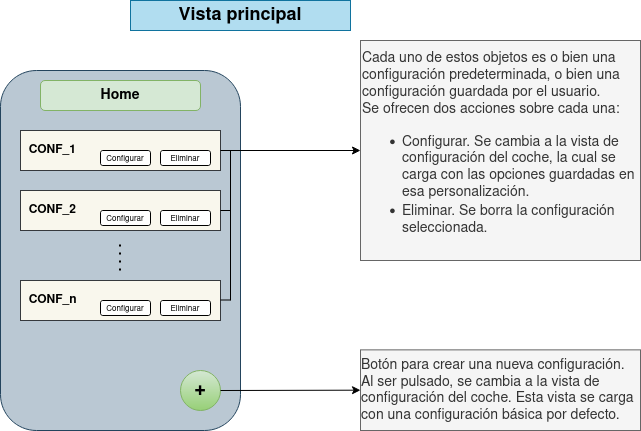
\includegraphics[scale=0.55]{imagenes/main_view.drawio.png}
\end{figure}

\begin{figure}[H]
\centering
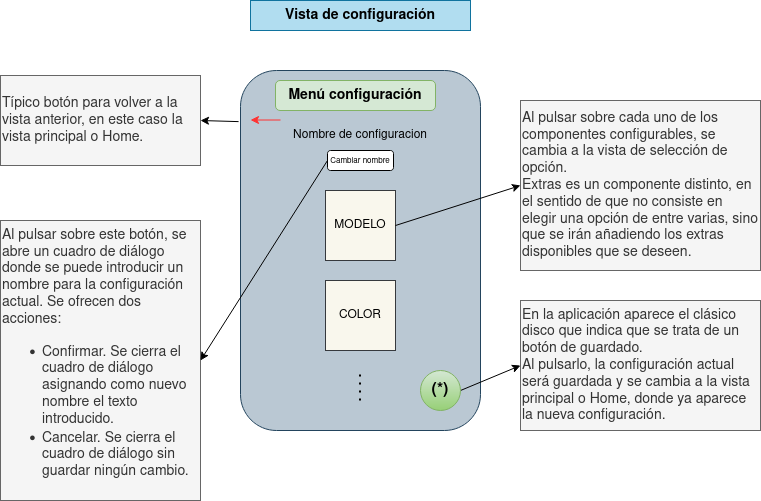
\includegraphics[scale=0.55]{imagenes/conf_view.drawio.png}
\end{figure}

\begin{figure}[H]
\centering
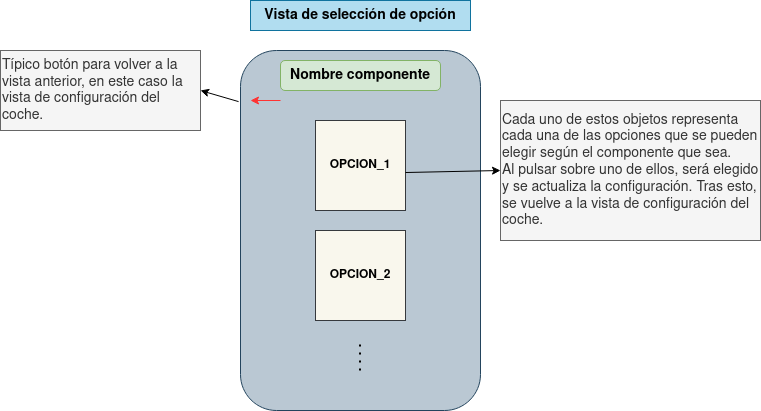
\includegraphics[scale=0.55]{imagenes/conf_componente_view.drawio.png}
\end{figure}

\newpage

%----------------------------------------------------------------------------------------
%	5. Diagrama de clases
%----------------------------------------------------------------------------------------

\section{Diagrama de clases}

%------------------------------------------------

\begin{figure}[H]
\centering
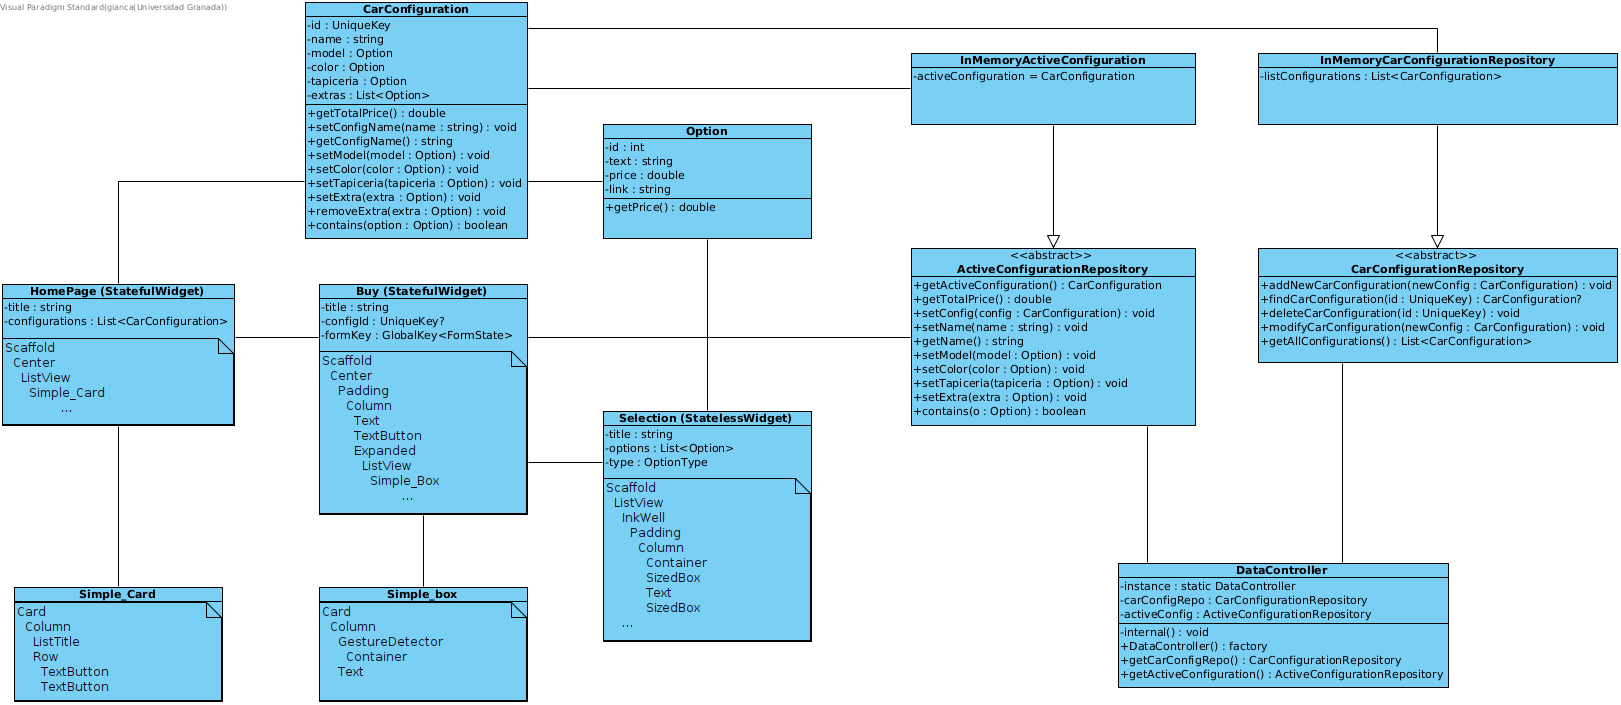
\includegraphics[scale=0.4]{imagenes/ds-diagramaclases.png}
\end{figure}

\newpage

%----------------------------------------------------------------------------------------
%	6. Patrones
%----------------------------------------------------------------------------------------

\section{Patrones}

\subsection{Patrón repositorio}

En este patrón buscamos modelar cómo vamos a manejar la persistencia de datos. Es una parte fundamental por los siguientes motivos:

\begin{itemize}
    \item En la aplicación, vamos a acceder constantemente a esta parte de persistencia de datos. Por tanto, para mantener un código limpio es fundamental que el acceso a la persistencia de datos sea cómoda y sencilla
    \item Es una parte que va a ser modificada. Ahora mismo solo modelamos esta persistencia de datos usando objetos en memoria. Pero en las siguientes prácticas, desarrollaremos una \emph{API Rest} para implementar esta persistencia de datos con una base de datos
    \item A la hora de escribir \emph{tests} en nuestra aplicación (cosa que no hemos hecho), es importante poder \emph{mockear} la persistencia de datos
\end{itemize}

Esto motiva el uso de patrón repositorio. Declaramos una interfaz que indica cómo se realizan las operaciones \emph{CRUD} de distintos conceptos de nuestra capa de negocio. Con esto, el acceso a estos datos es uniformizado y simplificado en toda la aplicación. Podemos tener distintas implementaciones para estas operaciones (ahora mismo solo tenemos objetos en memoria, pero con ese patrón es muy fácil implementar el acceso a una base de datos, a una \emph{API REST}, \ldots)
\\\\
Además, a la hora de implementar un \emph{mock}, solo tenemos que realizar una implementación de la interfaz. De hecho, los objetos que tenemos almacenados en memoria para nuestra aplicación sirven como un futuro \emph{mock}.
\\\\
Mostramos el código que implementa esta patrón en las siguientes figuras:

\begin{figure}[H]
    \centering
    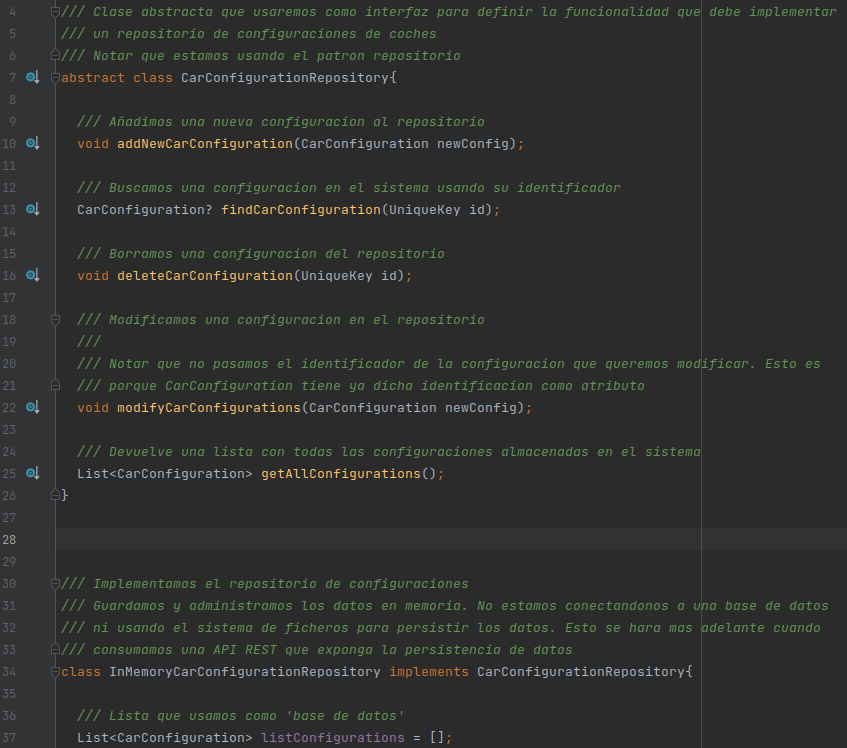
\includegraphics[scale=0.55]{imagenes/ds-repository1.png}
\end{figure}
\begin{figure}[H]
    \centering
    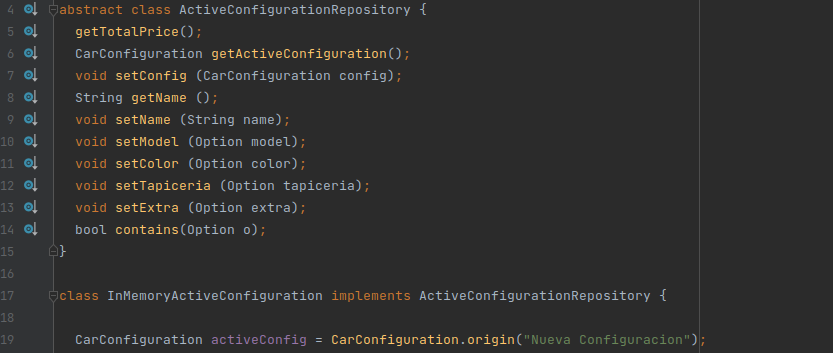
\includegraphics[scale=0.55]{imagenes/ds-repository2.png}
\end{figure}

\newpage

\subsection{Patrón \emph{singleton}}

Con el patrón anterior hemos modelado el acceso a los datos. Sin embargo, hasta ahora, esto puede ser un poco molesto. La opción directa para usar estas implementaciones en distinta partes de la aplicación, es inicializarlas en la función principal e ir pasando estas implementaciones por parámetro, por toda la aplicación.
\\\\
Esto es un problema en el caso que tengamos muchos repositorios distintos que ir pasando por toda la aplicación. Por tanto, pensamos que es adecuado el uso del patrón \emph{Singleton}. En dicho \emph{singleton}, que en nuestra código es la clase \emph{DataController}, se recogen todas las interfaces tipo repositorio, se inicializan con cierta implementación deseada y se ponen a disposición con \emph{getters}.
\\\\
De esta forma, si una parte de la aplicación necesita acceder a algún repositorio, puede crear un nuevo objeto de la clase (para lo que solo necesitamos un \emph{import '\ldots'} en el fichero) y acceder al repositorio adecuado.
\\\\
Mostramos el código que implementa este patrón en las siguientes figuras:

\begin{figure}[H]
    \centering
    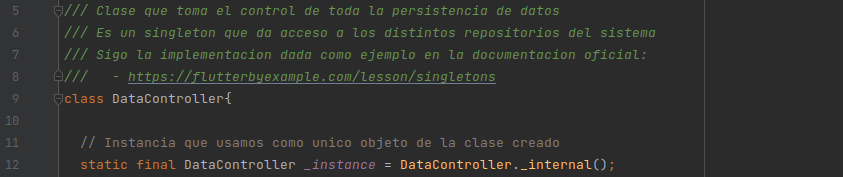
\includegraphics[scale=0.6]{imagenes/ds-singleton1.png}
\end{figure}
\begin{figure}[H]
    \centering
    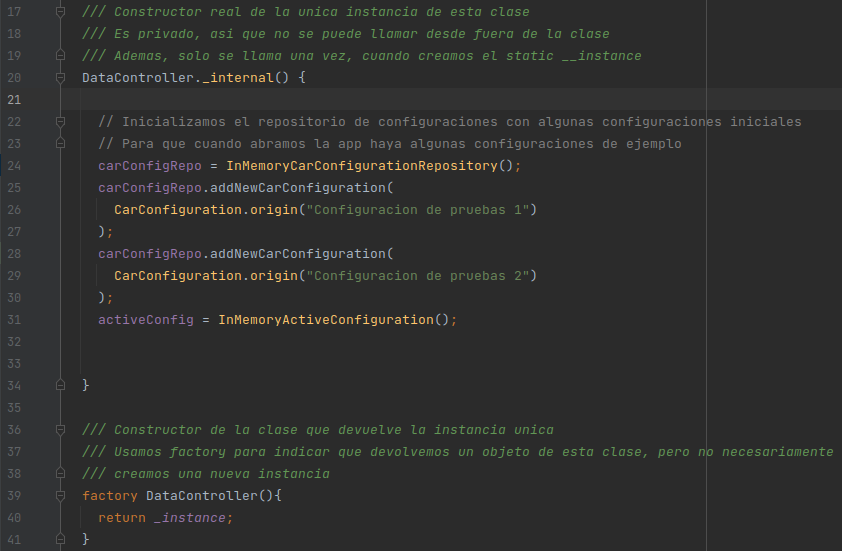
\includegraphics[scale=0.6]{imagenes/ds-singleton2.png}
\end{figure}

En estas figuras se puede apreciar que hemos implementado manualmente el patrón. Dart no trae por defecto el patrón, pero es muy sencillo de implementar, haciendo que el constructor devuelva un atributo estático.

\newpage

\subsection{Otros patrones}

Impuesto por \emph{Flutter}, estamos usando constantemente el patrón \emph{composite}. Estamos componiendo \emph{widgets} dentro de otros \emph{widgets} para crear las vistas.
\\\\
En segundo lugar, buscamos reusar todo el código posible para la creación de las vista. Esto lo hacemos en el módulo de componentes, donde implementamos una serie de funciones para crear componentes que usamos a lo largo de toda la aplicación. Con esto evitamos repetir el mismo código varias veces y, más importante, mantenemos una interfaz visual uniforme. Si queremos cambiar el \emph{look \& feel} de la aplicación, podemos cambiar estas funciones y automáticamente cambiará casi toda la interfaz gráfica de la aplicación.
\\\\
En parte estamos implementando el patrón \emph{Modelo - Vista - Controlador}, aunque sin el controlador. Tenemos un modelo para la configuración del coche, que interactúa con la parte de persistencia de datos y con las vistas de la aplicación.

\newpage

\section{Uso de \emph{Github}}

Como sistema de control de versiones hemos usado \emph{Github}. Para organizar el trabajo, hemos usado los siguientes procedimientos:

\begin{itemize}
    \item Uso de \emph{issues} para marcar las tareas a completar. También hemos usado \emph{issues} para discutir sobre distintos patrones a usar
    \item Uso de ramas para desarrollar código en paralelo. Con \emph{pull requests} revisamos y añadimos el código a la rama principal del repositorio
\end{itemize}

El repositorio se puede encontrar en \href{https://github.com/fervalnav/CarConfigurator}{https://github.com/fervalnav/CarConfigurator}.

\end{document}
